% !TeX spellcheck = en_GB
\section{Evaluation}
\subsection{Calibration}
\subsubsection{Laser Power}

\begin{figure}
	\centering
	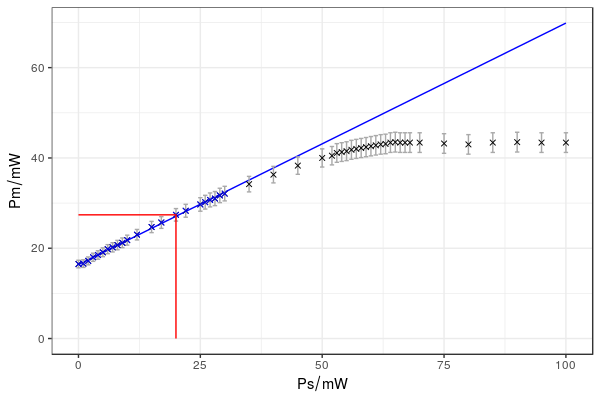
\includegraphics[width=\textwidth]{../figures/powercal.png}
	\caption{Measurement of the laser power}
	\label{fig:power}
\end{figure}

\subsubsection{Optical Spectrometer}
\begin{figure}
	\centering
	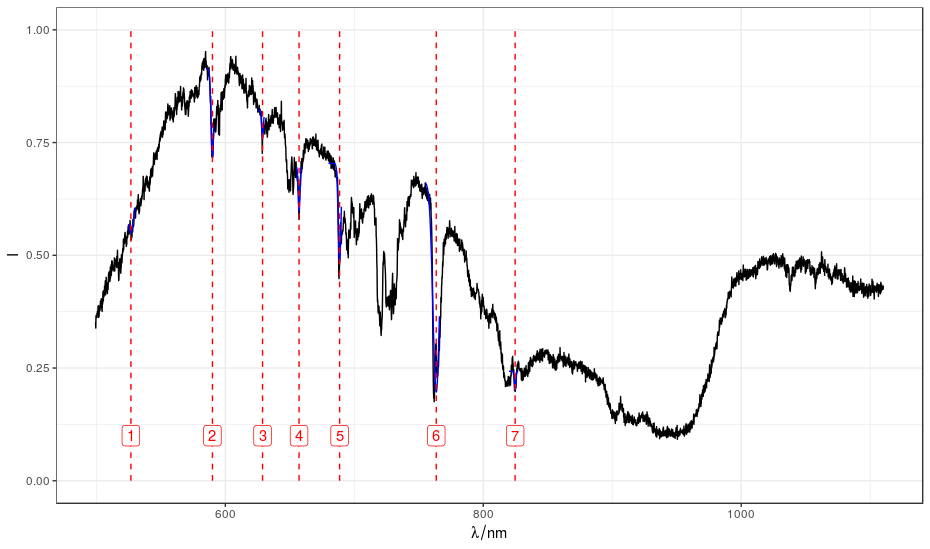
\includegraphics[width=\textwidth]{../figures/sunspectrum.png}
	\caption[Spectrum of the sun with identified Fraunhofer lines]{Spectrum of the sun with identified Fraunhofer lines for calibration of the optical spectrometer}
	\label{fig:sunspectrum}
\end{figure}

\begin{table}
	\centering
	\begin{tabular}{c|c|c|c|c}
		Peak&Position&Element&Position \cite{fraunhoferlines}&Difference\\
		1&$526.8\pm1.7$&Fe I&527.0&$-0.2$\\
		2&$590.0\pm0.5$&Na I&589.6&$+0.4$\\
		3&$628.9\pm0.3$&Fe I&630.3&$-1.4$\\
		4&$657.2\pm0.3$&H $\alpha$&656.3&$+0.9$\\
		5&$688.6\pm0.5$&&&\\
		6&$763.5\pm1.3$&&&\\
		7&$824.7\pm0.3$&&&\\
	\end{tabular}
	\caption{Positions of the Fraunhofer Lines compared to the literature values}
	\label{tab:fraunhofer}
\end{table}

\begin{figure}
	\centering
	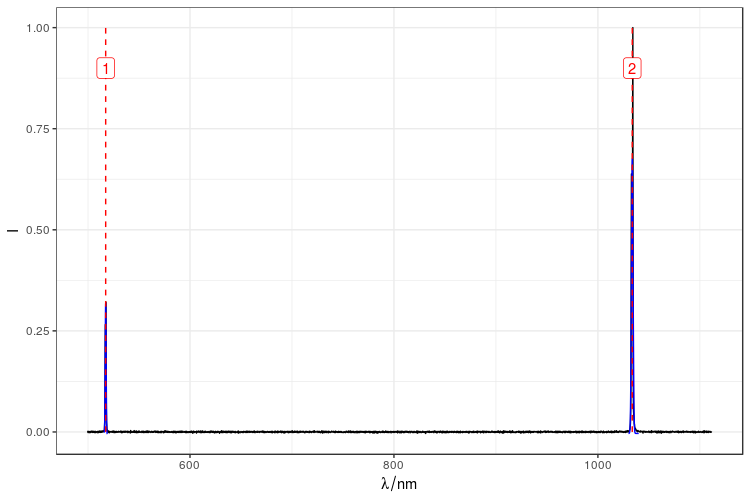
\includegraphics[width=\textwidth]{../figures/laserspectrum.png}
	\caption[Spectrum of the laser]{Spectrum of the laser with identified peaks at the wavelengths $\lambda=(517.3\pm0.2)\,\mathrm{nm}$ and $\lambda=(1033.7\pm0.4)\,\mathrm{nm}$}
	\label{fig:laserspectrum}
\end{figure}

\subsubsection{ODMR calibrations}
\paragraph{Shielding}
\begin{figure}
	\begin{subfigure}{0.5\textwidth}
		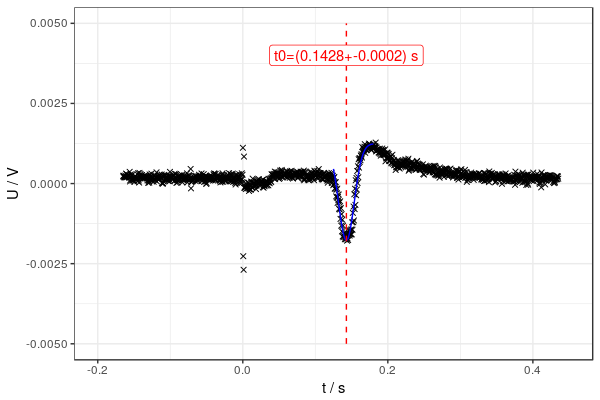
\includegraphics[width=\textwidth]{../figures/odmr-cal-1.png}
		\subcaption{without shielding}
	\end{subfigure}
		\begin{subfigure}{0.5\textwidth}	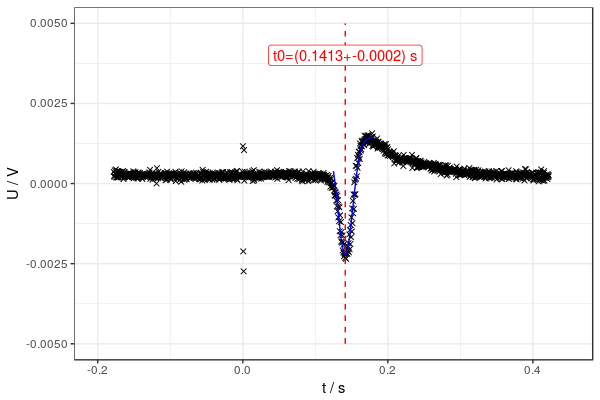
\includegraphics[width=\textwidth]{../figures/odmr-cal-2.png}
		\subcaption{with shielding}
	\end{subfigure}
	\caption{ODMR spectrum}
	\label{fig:odmr-shield}
\end{figure}
\paragraph{Time-to-Frequency Conversion}

\begin{figure}
	\begin{subfigure}{0.5\textwidth}
		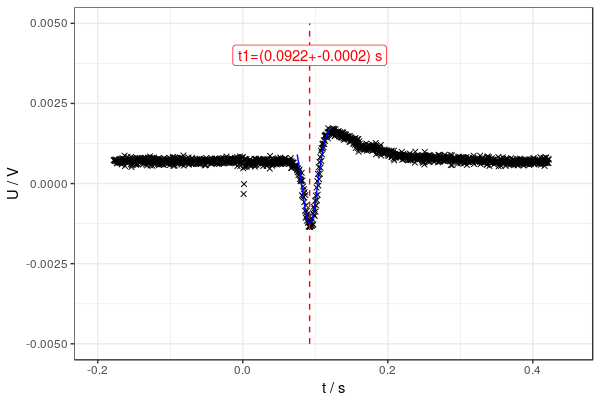
\includegraphics[width=\textwidth]{../figures/odmr-cal-4.png}
		\subcaption{shifted to the left}
	\end{subfigure}
	\begin{subfigure}{0.5\textwidth}
		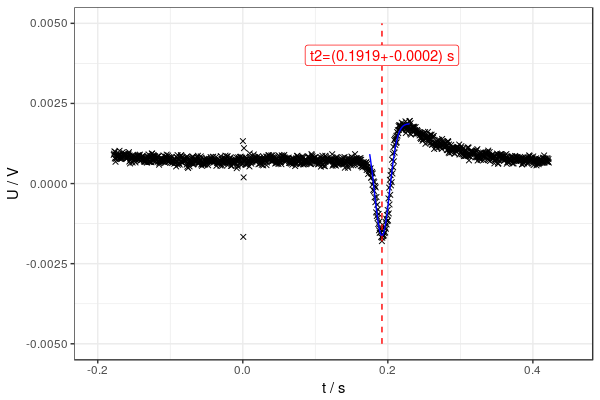
\includegraphics[width=\textwidth]{../figures/odmr-cal-3.png}
		\subcaption{shifted to the right}
	\end{subfigure}
	\caption{ODMR spectrum for time-to-frequency calibration}
	\label{fig:odmr-shift}
\end{figure}

Performing ODMR measurements we achieve the ODMR spectra on the oscilloscope. Therefore the spectra are time-resolved. To gain frequency-resolved spectra we need to calculate the conversion factor from time to frequency. We do this by performing two sweeps with shifted centre frequencies which allows us to calculate the conversion factor and also the offset since we know the frequency at which the peak appears.

The conversion can be expressed by the following equation:

\begin{align}
	f(t)&=\frac{f(t_1)(t_1-t_2)-(f(t_1)-f(t_2))t_1}{t_1-t_2}+\frac{f(t_1)-f(t_2)}{t_1-t_2}\cdot t
\end{align}

Inserting the values achieved from figure \ref{fig:odmr-shift} we get the following conversion function:

\begin{align}
	f(t)&=(1.003\pm0.003)\,\mathrm{\frac{GHz}{s}}\cdot t+(2.708\pm0.011)\,\mathrm{GHz}
\end{align}

Later in this document all spectra are converted by this function and therefore shown in the frequency domain. The errors are gained from the fit and propagated using Gaussian error propagation.

\subsection{Size of the Diamonds}

\subsection{Fluorescence Spectrum}
\begin{figure}
	\centering
	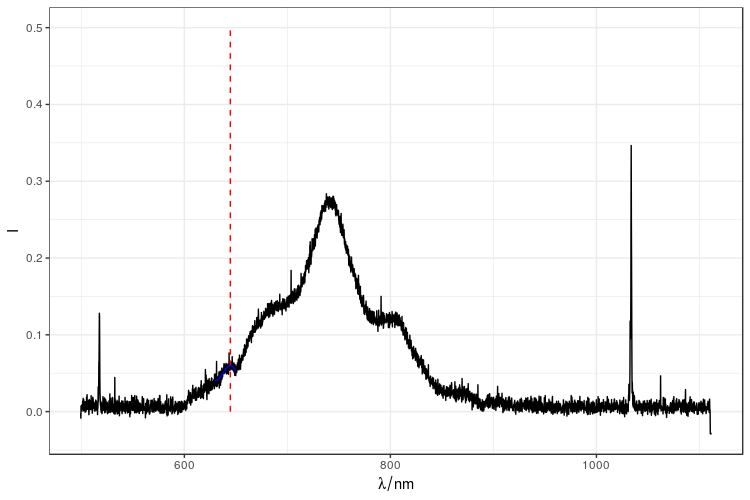
\includegraphics[width=\textwidth]{../figures/fluorescence.png}
	\caption[Fluorescence spectrum of the diamond]{Fluorescence spectrum of the diamond with the zero phonon line (red line) at $\lambda=(645\pm3)\,\mathrm{nm}$. The spectrum was achieved by averaging over 10 measurements.}
	\label{fig:fluorescence}
\end{figure}

\subsection{ODMR Measurements}
\begin{figure}
	\centering
	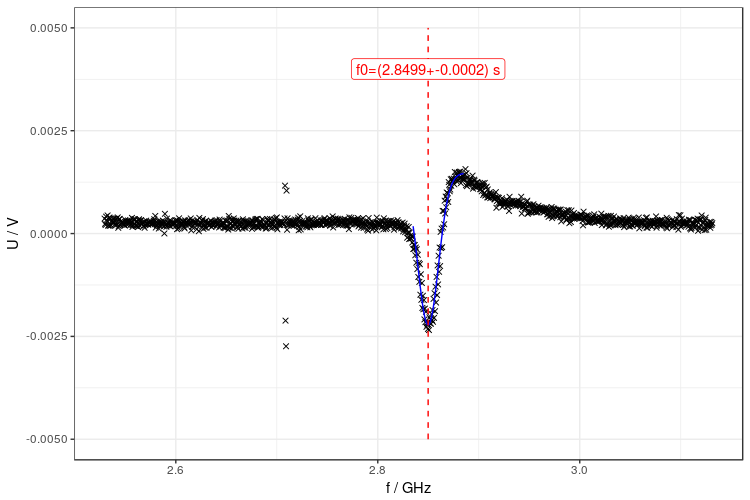
\includegraphics[width=0.8\textwidth]{../figures/odmr-1.png}
	\caption{ODMR Measurement of the diamond without B-Field}
	\label{fig:odmr-no-B}
\end{figure}